% Options for packages loaded elsewhere
\PassOptionsToPackage{unicode}{hyperref}
\PassOptionsToPackage{hyphens}{url}
\PassOptionsToPackage{dvipsnames,svgnames,x11names}{xcolor}
%
\documentclass[
  letterpaper,
  DIV=11,
  numbers=noendperiod]{scrartcl}

\usepackage{amsmath,amssymb}
\usepackage{lmodern}
\usepackage{iftex}
\ifPDFTeX
  \usepackage[T1]{fontenc}
  \usepackage[utf8]{inputenc}
  \usepackage{textcomp} % provide euro and other symbols
\else % if luatex or xetex
  \usepackage{unicode-math}
  \defaultfontfeatures{Scale=MatchLowercase}
  \defaultfontfeatures[\rmfamily]{Ligatures=TeX,Scale=1}
\fi
% Use upquote if available, for straight quotes in verbatim environments
\IfFileExists{upquote.sty}{\usepackage{upquote}}{}
\IfFileExists{microtype.sty}{% use microtype if available
  \usepackage[]{microtype}
  \UseMicrotypeSet[protrusion]{basicmath} % disable protrusion for tt fonts
}{}
\makeatletter
\@ifundefined{KOMAClassName}{% if non-KOMA class
  \IfFileExists{parskip.sty}{%
    \usepackage{parskip}
  }{% else
    \setlength{\parindent}{0pt}
    \setlength{\parskip}{6pt plus 2pt minus 1pt}}
}{% if KOMA class
  \KOMAoptions{parskip=half}}
\makeatother
\usepackage{xcolor}
\setlength{\emergencystretch}{3em} % prevent overfull lines
\setcounter{secnumdepth}{-\maxdimen} % remove section numbering
% Make \paragraph and \subparagraph free-standing
\ifx\paragraph\undefined\else
  \let\oldparagraph\paragraph
  \renewcommand{\paragraph}[1]{\oldparagraph{#1}\mbox{}}
\fi
\ifx\subparagraph\undefined\else
  \let\oldsubparagraph\subparagraph
  \renewcommand{\subparagraph}[1]{\oldsubparagraph{#1}\mbox{}}
\fi


\providecommand{\tightlist}{%
  \setlength{\itemsep}{0pt}\setlength{\parskip}{0pt}}\usepackage{longtable,booktabs,array}
\usepackage{calc} % for calculating minipage widths
% Correct order of tables after \paragraph or \subparagraph
\usepackage{etoolbox}
\makeatletter
\patchcmd\longtable{\par}{\if@noskipsec\mbox{}\fi\par}{}{}
\makeatother
% Allow footnotes in longtable head/foot
\IfFileExists{footnotehyper.sty}{\usepackage{footnotehyper}}{\usepackage{footnote}}
\makesavenoteenv{longtable}
\usepackage{graphicx}
\makeatletter
\def\maxwidth{\ifdim\Gin@nat@width>\linewidth\linewidth\else\Gin@nat@width\fi}
\def\maxheight{\ifdim\Gin@nat@height>\textheight\textheight\else\Gin@nat@height\fi}
\makeatother
% Scale images if necessary, so that they will not overflow the page
% margins by default, and it is still possible to overwrite the defaults
% using explicit options in \includegraphics[width, height, ...]{}
\setkeys{Gin}{width=\maxwidth,height=\maxheight,keepaspectratio}
% Set default figure placement to htbp
\makeatletter
\def\fps@figure{htbp}
\makeatother

\usepackage{amsmath}
\usepackage{booktabs}
\usepackage{caption}
\usepackage{longtable}
\usepackage{fontspec}
\usepackage{multirow}
\usepackage{multicol}
\usepackage{colortbl}
\usepackage{hhline}
\newlength\Oldarrayrulewidth
\newlength\Oldtabcolsep
\usepackage{array}
\usepackage{hyperref}
\usepackage{float}
\usepackage{wrapfig}
\usepackage{tabularray}
\usepackage[normalem]{ulem}
\usepackage{graphicx}
\UseTblrLibrary{booktabs}
\UseTblrLibrary{rotating}
\UseTblrLibrary{siunitx}
\NewTableCommand{\tinytableDefineColor}[3]{\definecolor{#1}{#2}{#3}}
\newcommand{\tinytableTabularrayUnderline}[1]{\underline{#1}}
\newcommand{\tinytableTabularrayStrikeout}[1]{\sout{#1}}
\KOMAoption{captions}{tableheading}
\makeatletter
\makeatother
\makeatletter
\makeatother
\makeatletter
\@ifpackageloaded{caption}{}{\usepackage{caption}}
\AtBeginDocument{%
\ifdefined\contentsname
  \renewcommand*\contentsname{Table of contents}
\else
  \newcommand\contentsname{Table of contents}
\fi
\ifdefined\listfigurename
  \renewcommand*\listfigurename{List of Figures}
\else
  \newcommand\listfigurename{List of Figures}
\fi
\ifdefined\listtablename
  \renewcommand*\listtablename{List of Tables}
\else
  \newcommand\listtablename{List of Tables}
\fi
\ifdefined\figurename
  \renewcommand*\figurename{Figure}
\else
  \newcommand\figurename{Figure}
\fi
\ifdefined\tablename
  \renewcommand*\tablename{Table}
\else
  \newcommand\tablename{Table}
\fi
}
\@ifpackageloaded{float}{}{\usepackage{float}}
\floatstyle{ruled}
\@ifundefined{c@chapter}{\newfloat{codelisting}{h}{lop}}{\newfloat{codelisting}{h}{lop}[chapter]}
\floatname{codelisting}{Listing}
\newcommand*\listoflistings{\listof{codelisting}{List of Listings}}
\makeatother
\makeatletter
\@ifpackageloaded{caption}{}{\usepackage{caption}}
\@ifpackageloaded{subcaption}{}{\usepackage{subcaption}}
\makeatother
\makeatletter
\@ifpackageloaded{tcolorbox}{}{\usepackage[many]{tcolorbox}}
\makeatother
\makeatletter
\@ifundefined{shadecolor}{\definecolor{shadecolor}{rgb}{.97, .97, .97}}
\makeatother
\makeatletter
\makeatother
\ifLuaTeX
  \usepackage{selnolig}  % disable illegal ligatures
\fi
\IfFileExists{bookmark.sty}{\usepackage{bookmark}}{\usepackage{hyperref}}
\IfFileExists{xurl.sty}{\usepackage{xurl}}{} % add URL line breaks if available
\urlstyle{same} % disable monospaced font for URLs
\hypersetup{
  pdftitle={Chapter Two: Clustering the Council},
  colorlinks=true,
  linkcolor={blue},
  filecolor={Maroon},
  citecolor={Blue},
  urlcolor={Blue},
  pdfcreator={LaTeX via pandoc}}

\title{Chapter Two: Clustering the Council}
\author{}
\date{}

\begin{document}
\maketitle
\ifdefined\Shaded\renewenvironment{Shaded}{\begin{tcolorbox}[frame hidden, interior hidden, enhanced, breakable, borderline west={3pt}{0pt}{shadecolor}, boxrule=0pt, sharp corners]}{\end{tcolorbox}}\fi

The New York City Council, at least since 2021, has been a body with a
high rate of cooperation, its members spend a lot of time supporting a
wide array of other member's bills. Additionally, there is a high rate
of agenda control; bills that will not pass a floor vote do not make it
to the floor, they die in committee. These aspects of the legislative
process combine to make looking at the legislative clusters of members
murky, so much cooperation can mask fault lines on the body. This
murkiness does not, however, mean those fault lines are not there. When
these two types of clustering, voting and sponsorship, are done in
unison, the same clusters emerge from both, revealing a group of
progressive legislators who manage to push through the relative
unanimity of the body to define a distinctly progressive legislative
agenda. This chapter will work through the clustering process, showing
the methodological considerations and the outcomes of both the voting
and sponsoring clustering process. It will then look to see how the
emergent progressive cluster is also reflected in the electoral
demographic data.

\hypertarget{voting}{%
\section{Voting}\label{voting}}

Council floor votes are heavily lopsided, most pass with only a few
dissenting conservative voices. This makes isolating the Council's
conservative's quite easy, but makes breaking the rest of the body into
clusters more difficult. To attempt to do this K-Means clustering, a
clustering methodology with wide application, which seeks to partition a
set of observations into a pre-defined number of clusters around
centroids that minimize within cluster variance, was employed
{[}@lloyd1982; @steinley2006{]}. The data used to cluster were all floor
votes from 2022 and 2023, reduced to the 100 closest votes with at least
30 members voting, measured by the ratio of anti-votes and abstentions
to pro votes. The votes were then one-hot coded, which makes dummy
variables for each option for each bill (e.g.~a dummy for pro bill 1, a
dummy for anti bill 1, etc.). I then ran the K-Means clustering on this
dataset. When running K-Means a number of clusters are defined in
advance, several common tests were used to predetermine the amount of
clusters as well as experimenting with the results. The best results
were obtained with five clusters, but no matter how many clusters were
defined the method pulls out the conservatives, who vote no or abstain
as a bloc on much legislation. If more than three cluster are defined,
it also pulls out a group of progressive council members including both
DSA members as well as other progressive stalwarts such as Chi Ossé,
Jennifer Guttierez, Sandy Nurse, and Shahana Hanif. Table 1 below shows
both the Conservative and Progressive caucus.

\begin{longtable}{rl}
\toprule
vote\_cluster & proper\_names \\ 
\midrule
0 & Rita C. Joseph, Julie Menin, Sandra Ung, Eric Dinowitz, Diana I. Ayala, Justin L. Brannan, Selvena N. Brooks-Powers, Christopher Marte, Nantasha M. Williams, Mercedes Narcisse, Carmen N. De La Rosa, Carlina Rivera, Shekar Krishnan, Marjorie Velázquez, Althea V.  Stevens, Lynn C. Schulman, James F. Gennaro, Pierina Ana Sanchez, Julie Won, Gale A. Brewer, Crystal Hudson, Shaun Abreu, Amanda Farías, Oswald Feliz, Rafael Salamanca, Jr., Linda Lee, Adrienne E. Adams, Keith Powers, Kamillah Hanks, Darlene Mealy, Francisco P. Moya, Erik D. Bottcher, Kevin C. Riley, Farah N. Louis \\ 
1 & Ari Kagan, David M. Carr, Inna Vernikov, Joann Ariola, Joseph C. Borelli, Vickie Paladino, Kalman Yeger, Robert F. Holden \\ 
2 & Kristin Richardson Jordan, Chi A. Ossé, Tiffany Cabán, Sandy Nurse, Alexa Avilés, Jennifer Gutiérrez, Charles Barron, Shahana K. Hanif, Lincoln Restler \\ 
\bottomrule
\end{longtable}

K-Means clustering with Sickit-Learn allows for examination of how each
item on which the clustering was performed (here, votes on bills)
affected the overall cluster placement. The bills that most influenced
the placement of these progressive members into a cluster are no votes
on budget bills and mayoral appointments (all of which nonetheless
passed). No matter how many more clusters are specified no new group
cluster forms; individuals from the massive non-progressive or
conservative cluster start to peel off one by one. There are three
voting clusters in the Council: a large majority that vote yes on most
bills for which they are present, and two dissenting minorities, a
conservative one who votes no quite frequently and a progressive one who
votes no on key pieces of legislation, especially in cases in which to
do so is antagonistic to the mayor. It is the latter that is of the most
interest to this project as it is a demonstration of the vying for
regime control described in Chapter 1. This portion of the council, loud
and active in its opposition to Mayor Adams's conservative policy
agenda, has helped push the entire body more firmly into is role of
Mayoral oversight, culminating in overridden vetoes and the Speaker
referring to the body as a ``co-equal'' branch of government
{[}@adams{]}.

\hypertarget{co-sponsorship}{%
\section{Co-Sponsorship}\label{co-sponsorship}}

Though examining sponsorship bills faces similar challenges, it reveals
similar groups of conservative and progressive legislators. Many bills,
especially those that pass, have high numbers of sponsors. The mean
number of sponsors for a bill in the dataset was 13, with the mean
number for a bill that passed was 23. Additionally, there is a lot of
co-sponsorship across ideological lines; every member has co-sponsored
with every other member at least once, often many more times than once.
This is perhaps not surprising, as Lincoln Restler pointed out to me
voters prize pragmatism in their council votes and members are aware of
this, so there is motivation to work across boundaries to get things
done {[}@restler2024{]}. This high rate of cooperation means that using
traditional methods to visualize networks leads to a large bird's nest
of co-sponsorship, a version of this tangled graph is included in the
appendix. Nonetheless, members do of course co-sponsor with some members
much more frequently than others, so despite the significant noise
caused by cooperation some patterns do emerge.

To identify these patterns, I began by once again employing K-Means
clustering. To prepare the data I made a matrix that described how often
each member co-sponsored with another, on a scale of 0-1, removing bills
that had 40 or more co-sponsors. I then ran the K-Means on this matrix.
The results of this are recorded in Table 2 below. The results mirror
those found in the voting patterns above, cluster 1 again features both
DSA members as well as other (though not all) members from the voting
clusters above. This cluster remained as long as there were more than
two clusters defined.

\begin{longtable}{rl}
\toprule
k\_spon & proper\_names \\ 
\midrule
0 & Rita C. Joseph, Julie Menin, Kristin Richardson Jordan, Sandra Ung, Eric Dinowitz, Diana I. Ayala, Justin L. Brannan, Selvena N. Brooks-Powers, Christopher Marte, Nantasha M. Williams, Mercedes Narcisse, Carmen N. De La Rosa, Carlina Rivera, Shekar Krishnan, Marjorie Velázquez, Althea V.  Stevens, Lynn C. Schulman, Chi A. Ossé, James F. Gennaro \\ 
1 & Pierina Ana Sanchez, Tiffany Cabán, Julie Won, Gale A. Brewer, Sandy Nurse, Crystal Hudson, Shaun Abreu, Amanda Farías, Alexa Avilés, Jennifer Gutiérrez \\ 
2 & Oswald Feliz, Rafael Salamanca, Jr., Linda Lee, Adrienne E. Adams, Keith Powers, Kamillah Hanks, Ari Kagan, Charles Barron, Darlene Mealy, Francisco P. Moya, Erik D. Bottcher \\ 
3 & Kevin C. Riley, Shahana K. Hanif, Farah N. Louis, Lincoln Restler \\ 
4 & David M. Carr, Inna Vernikov, Joann Ariola, Joseph C. Borelli, Vickie Paladino \\ 
5 & Kalman Yeger, Robert F. Holden \\ 
\bottomrule
\end{longtable}

The Louvain method of community detection was used to check the
robustness of the K-Means results. This algorithm takes data that has
already been structured for network mapping (different than the matrix
used for the K-Means) and detects communities based on the weights of
the edges. Here clusters are not predefined, the algorithm arrives at a
number on its own. This method of community detection has seen
increasing application in Political Science research, including a
similar task of detecting small and nuanced communities in
co-sponsorship of bills in the UN General Assembly {[}@meyer2021{]}. The
results are displayed in Table 3 below, where the the Louvain method
picks up a similar group of progressives, though with many more
additions than the method above.

\global\setlength{\Oldarrayrulewidth}{\arrayrulewidth}

\global\setlength{\Oldtabcolsep}{\tabcolsep}

\setlength{\tabcolsep}{2pt}

\renewcommand*{\arraystretch}{1.5}



\providecommand{\ascline}[3]{\noalign{\global\arrayrulewidth #1}\arrayrulecolor[HTML]{#2}\cline{#3}}

\begin{longtable}[c]{|p{0.57in}|p{24.54in}}



\ascline{1.5pt}{666666}{1-2}

\multicolumn{1}{>{\raggedleft}m{\dimexpr 0.57in+0\tabcolsep}}{\textcolor[HTML]{000000}{\fontsize{11}{11}\selectfont{\global\setmainfont{Arial}{louv}}}} & \multicolumn{1}{>{\raggedright}m{\dimexpr 24.54in+0\tabcolsep}}{\textcolor[HTML]{000000}{\fontsize{11}{11}\selectfont{\global\setmainfont{Arial}{proper\_names}}}} \\

\ascline{1.5pt}{666666}{1-2}\endfirsthead 

\ascline{1.5pt}{666666}{1-2}

\multicolumn{1}{>{\raggedleft}m{\dimexpr 0.57in+0\tabcolsep}}{\textcolor[HTML]{000000}{\fontsize{11}{11}\selectfont{\global\setmainfont{Arial}{louv}}}} & \multicolumn{1}{>{\raggedright}m{\dimexpr 24.54in+0\tabcolsep}}{\textcolor[HTML]{000000}{\fontsize{11}{11}\selectfont{\global\setmainfont{Arial}{proper\_names}}}} \\

\ascline{1.5pt}{666666}{1-2}\endhead



\multicolumn{1}{>{\raggedleft}m{\dimexpr 0.57in+0\tabcolsep}}{\textcolor[HTML]{000000}{\fontsize{11}{11}\selectfont{\global\setmainfont{Arial}{0}}}} & \multicolumn{1}{>{\raggedright}m{\dimexpr 24.54in+0\tabcolsep}}{\textcolor[HTML]{000000}{\fontsize{11}{11}\selectfont{\global\setmainfont{Arial}{Rita\ C.\ Joseph,\ Kristin\ Richardson\ Jordan,\ Christopher\ Marte,\ Carmen\ N.\ De\ La\ Rosa,\ Carlina\ Rivera,\ Shekar\ Krishnan,\ Chi\ A.\ Ossé,\ Tiffany\ Cabán,\ Julie\ Won,\ Gale\ A.\ Brewer,\ Sandy\ Nurse,\ Crystal\ Hudson,\ Shaun\ Abreu,\ Amanda\ Farías,\ Alexa\ Avilés,\ Jennifer\ Gutiérrez,\ Adrienne\ E.\ Adams,\ Shahana\ K.\ Hanif,\ Lincoln\ Restler}}}} \\





\multicolumn{1}{>{\raggedleft}m{\dimexpr 0.57in+0\tabcolsep}}{\textcolor[HTML]{000000}{\fontsize{11}{11}\selectfont{\global\setmainfont{Arial}{1}}}} & \multicolumn{1}{>{\raggedright}m{\dimexpr 24.54in+0\tabcolsep}}{\textcolor[HTML]{000000}{\fontsize{11}{11}\selectfont{\global\setmainfont{Arial}{Julie\ Menin,\ Eric\ Dinowitz,\ Justin\ L.\ Brannan,\ Selvena\ N.\ Brooks-Powers,\ Althea\ V.\ \ Stevens,\ James\ F.\ Gennaro,\ Oswald\ Feliz,\ Rafael\ Salamanca,\ Jr.,\ Keith\ Powers,\ Kamillah\ Hanks,\ Ari\ Kagan,\ Charles\ Barron,\ Francisco\ P.\ Moya,\ Farah\ N.\ Louis,\ David\ M.\ Carr,\ Inna\ Vernikov,\ Joann\ Ariola,\ Joseph\ C.\ Borelli,\ Vickie\ Paladino,\ Kalman\ Yeger,\ Robert\ F.\ Holden}}}} \\





\multicolumn{1}{>{\raggedleft}m{\dimexpr 0.57in+0\tabcolsep}}{\textcolor[HTML]{000000}{\fontsize{11}{11}\selectfont{\global\setmainfont{Arial}{2}}}} & \multicolumn{1}{>{\raggedright}m{\dimexpr 24.54in+0\tabcolsep}}{\textcolor[HTML]{000000}{\fontsize{11}{11}\selectfont{\global\setmainfont{Arial}{Sandra\ Ung,\ Diana\ I.\ Ayala,\ Nantasha\ M.\ Williams,\ Mercedes\ Narcisse,\ Marjorie\ Velázquez,\ Lynn\ C.\ Schulman,\ Pierina\ Ana\ Sanchez,\ Linda\ Lee,\ Darlene\ Mealy,\ Erik\ D.\ Bottcher,\ Kevin\ C.\ Riley}}}} \\

\ascline{1.5pt}{666666}{1-2}



\end{longtable}



\arrayrulecolor[HTML]{000000}

\global\setlength{\arrayrulewidth}{\Oldarrayrulewidth}

\global\setlength{\tabcolsep}{\Oldtabcolsep}

\renewcommand*{\arraystretch}{1}

Despite some variation in its specific makeup, both methods agree that
there is a progressive bloc sponsoring together and voting in protest
together. To try and make sense of these similar but slightly different
clustering blocs, two different methods of meta-clustering the three
types of clusters already done were employed. One was a repeat of the
K-Means after again one-hot encoding the data. The other was K-Mode,
which, as the name suggests, is a similar method of clustering that
takes the mode rather than the mean to handle categorical data. While
the two methods diverged on some members, they agreed exactly on the
progressive group. Table 4 shows this group.

\begin{longtable}{rl}
\toprule
kmode\_cluster & proper\_names \\ 
\midrule
3 & Kristin Richardson Jordan, Chi A. Ossé, Tiffany Cabán, Sandy Nurse, Alexa Avilés, Jennifer Gutiérrez, Shahana K. Hanif, Lincoln Restler \\ 
\bottomrule
\end{longtable}

\hypertarget{sponsored-bills}{%
\section{Sponsored Bills}\label{sponsored-bills}}

The bills these progressives co-sponsor fall into two general
categories, bills that attract a high-rate of fellow progressives and
have a low chance of passing, and bills that are primarily sponsored by
progressives but attract a wider level of support and therefore have a
higher chance of passing. Both groups of bills track closely with the
egalitarian urban order defined by Weaver and discussed in Chapter 1.
Table 5 shows the bills which have the highest percentage of sponsors
from the progressive cluster. They concern worker protections, oversight
of the NYPD, tenant advocacy, environmental concerns, college counseling
for low-income New Yorkers and protections for cyclists. Not a single
bill with more than 60\% of its sponsors from this cluster was enacted,
so while these progressive-heavy bills may be pushing the rhetoric of
the council left they have not, as of yet, translated into legislation.

\begin{longtable}{lr}
\toprule
EventItemMatterName & percent\_cluster\_3 \\ 
\midrule
Requiring the police department to submit to the council reports of services provided to any private entity. & 100 \\ 
Establishing a pilot program to provide bleeding control training and kits. & 100 \\ 
Developing a college admissions counseling program. & 100 \\ 
Requiring a study and mitigation of the impacts of methane gas emissions on city trees. & 100 \\ 
Requiring low-wage workers to enter into covenants not to compete and also to require employers to notify potential employees of any requirement to enter into a covenant not to compete. & 100 \\ 
Creation of a residential parking permit system in Sunset Park and Red Hook. & 100 \\ 
Requiring building owners to provide information on elected officials to tenants in multiple dwellings. & 100 \\ 
Requiring taxis and for-hire vehicles to display a decal warning passengers to look for cyclists when opening the door. & 100 \\ 
Enhancing penalties for sidewalk parking and installing bollards in M1 zoning districts. & 80 \\ 
Wrongful discharge from employment. & 80 \\ 
\bottomrule
\end{longtable}

This does not mean, however, that the group is ineffective. Dozens of
bills sponsored by members of this progressive cluster have been enacted
on topics that are slightly different but similarly progressive. Table 6
below shows the enacted cluster 3 bills with the highest rate of
co-sponsorship, a full list of bills they have passed are available in
the appendix. These bills have to do again with worker protections,
migrant rights, the distribution of free menstrual products, the
protections of LGBTQ New Yorkers, the protection of reproduction rights,
protections for the homeless, and a ``Marshall Plan for Moms'' to help
support working mothers. These members have clearly set a progressive
agenda both in practice and in rhetoric. To compare these bills to those
sponsored by other clusters, Table 7 shows a Term Frequency -- Inverse
Document Frequency (TF-IDF) of the text descriptions of the bills
sponsored by each group. What this in effect shows are the words that
occur most frequently in each groups legislation but less in others.

\begin{longtable}{lr}
\toprule
EventItemMatterName & percent\_cluster\_3 \\ 
\midrule
A biotechnology credit against the general corporation tax, the unincorporated business tax, and the corporate tax of 2015. & 50.00000 \\ 
Workers’ bill of rights and outreach to immigrant workers. & 40.00000 \\ 
Requiring reports on removals involving individuals experiencing homelessness and the outcomes for those individuals. & 36.36364 \\ 
Menstrual Products & 35.71429 \\ 
Prohibiting the use of city resources to enforce abortion restrictions. & 33.33333 \\ 
DOITT updating 311 complaint types and reporting on such updates. & 28.57143 \\ 
Providing food delivery workers with information on safety measures that mitigate the fire risks posed by powered mobility devices. & 28.57143 \\ 
Establishment of a Marshall plan for moms task force to develop and issue recommendations on how to support working mothers, other parents, and caregivers. & 26.66667 \\ 
Requiring the commissioner of cultural affairs to report annually on department funding of art and cultural organizations and institutions. & 26.31579 \\ 
Report on the provision of medical services related to reproductive health care. & 26.08696 \\ 
\bottomrule
\end{longtable}

\global\setlength{\Oldarrayrulewidth}{\arrayrulewidth}

\global\setlength{\Oldtabcolsep}{\tabcolsep}

\setlength{\tabcolsep}{2pt}

\renewcommand*{\arraystretch}{1.5}



\providecommand{\ascline}[3]{\noalign{\global\arrayrulewidth #1}\arrayrulecolor[HTML]{#2}\cline{#3}}

\begin{longtable}[c]{|p{0.75in}|p{0.75in}|p{0.75in}|p{0.75in}|p{0.75in}|p{0.75in}|p{0.75in}|p{0.75in}|p{0.75in}|p{0.75in}|p{0.75in}|p{0.75in}}



\ascline{1.5pt}{666666}{1-12}

\multicolumn{1}{>{\raggedleft}m{\dimexpr 0.75in+0\tabcolsep}}{\textcolor[HTML]{000000}{\fontsize{11}{11}\selectfont{\global\setmainfont{Arial}{Cluster}}}} & \multicolumn{1}{>{\raggedright}m{\dimexpr 0.75in+0\tabcolsep}}{\textcolor[HTML]{000000}{\fontsize{11}{11}\selectfont{\global\setmainfont{Arial}{Word\ 1}}}} & \multicolumn{1}{>{\raggedright}m{\dimexpr 0.75in+0\tabcolsep}}{\textcolor[HTML]{000000}{\fontsize{11}{11}\selectfont{\global\setmainfont{Arial}{Word\ 2}}}} & \multicolumn{1}{>{\raggedright}m{\dimexpr 0.75in+0\tabcolsep}}{\textcolor[HTML]{000000}{\fontsize{11}{11}\selectfont{\global\setmainfont{Arial}{Word\ 3}}}} & \multicolumn{1}{>{\raggedright}m{\dimexpr 0.75in+0\tabcolsep}}{\textcolor[HTML]{000000}{\fontsize{11}{11}\selectfont{\global\setmainfont{Arial}{Word\ 4}}}} & \multicolumn{1}{>{\raggedright}m{\dimexpr 0.75in+0\tabcolsep}}{\textcolor[HTML]{000000}{\fontsize{11}{11}\selectfont{\global\setmainfont{Arial}{Word\ 5}}}} & \multicolumn{1}{>{\raggedright}m{\dimexpr 0.75in+0\tabcolsep}}{\textcolor[HTML]{000000}{\fontsize{11}{11}\selectfont{\global\setmainfont{Arial}{Word\ 6}}}} & \multicolumn{1}{>{\raggedright}m{\dimexpr 0.75in+0\tabcolsep}}{\textcolor[HTML]{000000}{\fontsize{11}{11}\selectfont{\global\setmainfont{Arial}{Word\ 7}}}} & \multicolumn{1}{>{\raggedright}m{\dimexpr 0.75in+0\tabcolsep}}{\textcolor[HTML]{000000}{\fontsize{11}{11}\selectfont{\global\setmainfont{Arial}{Word\ 8}}}} & \multicolumn{1}{>{\raggedright}m{\dimexpr 0.75in+0\tabcolsep}}{\textcolor[HTML]{000000}{\fontsize{11}{11}\selectfont{\global\setmainfont{Arial}{Word\ 9}}}} & \multicolumn{1}{>{\raggedright}m{\dimexpr 0.75in+0\tabcolsep}}{\textcolor[HTML]{000000}{\fontsize{11}{11}\selectfont{\global\setmainfont{Arial}{Word\ 10}}}} & \multicolumn{1}{>{\raggedright}m{\dimexpr 0.75in+0\tabcolsep}}{\textcolor[HTML]{000000}{\fontsize{11}{11}\selectfont{\global\setmainfont{Arial}{Word\ 11}}}} \\

\ascline{1.5pt}{666666}{1-12}\endfirsthead 

\ascline{1.5pt}{666666}{1-12}

\multicolumn{1}{>{\raggedleft}m{\dimexpr 0.75in+0\tabcolsep}}{\textcolor[HTML]{000000}{\fontsize{11}{11}\selectfont{\global\setmainfont{Arial}{Cluster}}}} & \multicolumn{1}{>{\raggedright}m{\dimexpr 0.75in+0\tabcolsep}}{\textcolor[HTML]{000000}{\fontsize{11}{11}\selectfont{\global\setmainfont{Arial}{Word\ 1}}}} & \multicolumn{1}{>{\raggedright}m{\dimexpr 0.75in+0\tabcolsep}}{\textcolor[HTML]{000000}{\fontsize{11}{11}\selectfont{\global\setmainfont{Arial}{Word\ 2}}}} & \multicolumn{1}{>{\raggedright}m{\dimexpr 0.75in+0\tabcolsep}}{\textcolor[HTML]{000000}{\fontsize{11}{11}\selectfont{\global\setmainfont{Arial}{Word\ 3}}}} & \multicolumn{1}{>{\raggedright}m{\dimexpr 0.75in+0\tabcolsep}}{\textcolor[HTML]{000000}{\fontsize{11}{11}\selectfont{\global\setmainfont{Arial}{Word\ 4}}}} & \multicolumn{1}{>{\raggedright}m{\dimexpr 0.75in+0\tabcolsep}}{\textcolor[HTML]{000000}{\fontsize{11}{11}\selectfont{\global\setmainfont{Arial}{Word\ 5}}}} & \multicolumn{1}{>{\raggedright}m{\dimexpr 0.75in+0\tabcolsep}}{\textcolor[HTML]{000000}{\fontsize{11}{11}\selectfont{\global\setmainfont{Arial}{Word\ 6}}}} & \multicolumn{1}{>{\raggedright}m{\dimexpr 0.75in+0\tabcolsep}}{\textcolor[HTML]{000000}{\fontsize{11}{11}\selectfont{\global\setmainfont{Arial}{Word\ 7}}}} & \multicolumn{1}{>{\raggedright}m{\dimexpr 0.75in+0\tabcolsep}}{\textcolor[HTML]{000000}{\fontsize{11}{11}\selectfont{\global\setmainfont{Arial}{Word\ 8}}}} & \multicolumn{1}{>{\raggedright}m{\dimexpr 0.75in+0\tabcolsep}}{\textcolor[HTML]{000000}{\fontsize{11}{11}\selectfont{\global\setmainfont{Arial}{Word\ 9}}}} & \multicolumn{1}{>{\raggedright}m{\dimexpr 0.75in+0\tabcolsep}}{\textcolor[HTML]{000000}{\fontsize{11}{11}\selectfont{\global\setmainfont{Arial}{Word\ 10}}}} & \multicolumn{1}{>{\raggedright}m{\dimexpr 0.75in+0\tabcolsep}}{\textcolor[HTML]{000000}{\fontsize{11}{11}\selectfont{\global\setmainfont{Arial}{Word\ 11}}}} \\

\ascline{1.5pt}{666666}{1-12}\endhead



\multicolumn{1}{>{\raggedleft}m{\dimexpr 0.75in+0\tabcolsep}}{\textcolor[HTML]{000000}{\fontsize{11}{11}\selectfont{\global\setmainfont{Arial}{0}}}} & \multicolumn{1}{>{\raggedright}m{\dimexpr 0.75in+0\tabcolsep}}{\textcolor[HTML]{000000}{\fontsize{11}{11}\selectfont{\global\setmainfont{Arial}{housing}}}} & \multicolumn{1}{>{\raggedright}m{\dimexpr 0.75in+0\tabcolsep}}{\textcolor[HTML]{000000}{\fontsize{11}{11}\selectfont{\global\setmainfont{Arial}{health}}}} & \multicolumn{1}{>{\raggedright}m{\dimexpr 0.75in+0\tabcolsep}}{\textcolor[HTML]{000000}{\fontsize{11}{11}\selectfont{\global\setmainfont{Arial}{establishment}}}} & \multicolumn{1}{>{\raggedright}m{\dimexpr 0.75in+0\tabcolsep}}{\textcolor[HTML]{000000}{\fontsize{11}{11}\selectfont{\global\setmainfont{Arial}{creating}}}} & \multicolumn{1}{>{\raggedright}m{\dimexpr 0.75in+0\tabcolsep}}{\textcolor[HTML]{000000}{\fontsize{11}{11}\selectfont{\global\setmainfont{Arial}{education}}}} & \multicolumn{1}{>{\raggedright}m{\dimexpr 0.75in+0\tabcolsep}}{\textcolor[HTML]{000000}{\fontsize{11}{11}\selectfont{\global\setmainfont{Arial}{provide}}}} & \multicolumn{1}{>{\raggedright}m{\dimexpr 0.75in+0\tabcolsep}}{\textcolor[HTML]{000000}{\fontsize{11}{11}\selectfont{\global\setmainfont{Arial}{buildings}}}} & \multicolumn{1}{>{\raggedright}m{\dimexpr 0.75in+0\tabcolsep}}{\textcolor[HTML]{000000}{\fontsize{11}{11}\selectfont{\global\setmainfont{Arial}{mental}}}} & \multicolumn{1}{>{\raggedright}m{\dimexpr 0.75in+0\tabcolsep}}{\textcolor[HTML]{000000}{\fontsize{11}{11}\selectfont{\global\setmainfont{Arial}{campaign}}}} & \multicolumn{1}{>{\raggedright}m{\dimexpr 0.75in+0\tabcolsep}}{\textcolor[HTML]{000000}{\fontsize{11}{11}\selectfont{\global\setmainfont{Arial}{correction}}}} & \multicolumn{1}{>{\raggedright}m{\dimexpr 0.75in+0\tabcolsep}}{\textcolor[HTML]{000000}{\fontsize{11}{11}\selectfont{\global\setmainfont{Arial}{package}}}} \\





\multicolumn{1}{>{\raggedleft}m{\dimexpr 0.75in+0\tabcolsep}}{\textcolor[HTML]{000000}{\fontsize{11}{11}\selectfont{\global\setmainfont{Arial}{1}}}} & \multicolumn{1}{>{\raggedright}m{\dimexpr 0.75in+0\tabcolsep}}{\textcolor[HTML]{000000}{\fontsize{11}{11}\selectfont{\global\setmainfont{Arial}{parking}}}} & \multicolumn{1}{>{\raggedright}m{\dimexpr 0.75in+0\tabcolsep}}{\textcolor[HTML]{000000}{\fontsize{11}{11}\selectfont{\global\setmainfont{Arial}{service}}}} & \multicolumn{1}{>{\raggedright}m{\dimexpr 0.75in+0\tabcolsep}}{\textcolor[HTML]{000000}{\fontsize{11}{11}\selectfont{\global\setmainfont{Arial}{vehicles}}}} & \multicolumn{1}{>{\raggedright}m{\dimexpr 0.75in+0\tabcolsep}}{\textcolor[HTML]{000000}{\fontsize{11}{11}\selectfont{\global\setmainfont{Arial}{street}}}} & \multicolumn{1}{>{\raggedright}m{\dimexpr 0.75in+0\tabcolsep}}{\textcolor[HTML]{000000}{\fontsize{11}{11}\selectfont{\global\setmainfont{Arial}{veteran}}}} & \multicolumn{1}{>{\raggedright}m{\dimexpr 0.75in+0\tabcolsep}}{\textcolor[HTML]{000000}{\fontsize{11}{11}\selectfont{\global\setmainfont{Arial}{notification}}}} & \multicolumn{1}{>{\raggedright}m{\dimexpr 0.75in+0\tabcolsep}}{\textcolor[HTML]{000000}{\fontsize{11}{11}\selectfont{\global\setmainfont{Arial}{electric}}}} & \multicolumn{1}{>{\raggedright}m{\dimexpr 0.75in+0\tabcolsep}}{\textcolor[HTML]{000000}{\fontsize{11}{11}\selectfont{\global\setmainfont{Arial}{fire}}}} & \multicolumn{1}{>{\raggedright}m{\dimexpr 0.75in+0\tabcolsep}}{\textcolor[HTML]{000000}{\fontsize{11}{11}\selectfont{\global\setmainfont{Arial}{requests}}}} & \multicolumn{1}{>{\raggedright}m{\dimexpr 0.75in+0\tabcolsep}}{\textcolor[HTML]{000000}{\fontsize{11}{11}\selectfont{\global\setmainfont{Arial}{force}}}} & \multicolumn{1}{>{\raggedright}m{\dimexpr 0.75in+0\tabcolsep}}{\textcolor[HTML]{000000}{\fontsize{11}{11}\selectfont{\global\setmainfont{Arial}{violations}}}} \\





\multicolumn{1}{>{\raggedleft}m{\dimexpr 0.75in+0\tabcolsep}}{\textcolor[HTML]{000000}{\fontsize{11}{11}\selectfont{\global\setmainfont{Arial}{2}}}} & \multicolumn{1}{>{\raggedright}m{\dimexpr 0.75in+0\tabcolsep}}{\textcolor[HTML]{000000}{\fontsize{11}{11}\selectfont{\global\setmainfont{Arial}{health}}}} & \multicolumn{1}{>{\raggedright}m{\dimexpr 0.75in+0\tabcolsep}}{\textcolor[HTML]{000000}{\fontsize{11}{11}\selectfont{\global\setmainfont{Arial}{mental}}}} & \multicolumn{1}{>{\raggedright}m{\dimexpr 0.75in+0\tabcolsep}}{\textcolor[HTML]{000000}{\fontsize{11}{11}\selectfont{\global\setmainfont{Arial}{food}}}} & \multicolumn{1}{>{\raggedright}m{\dimexpr 0.75in+0\tabcolsep}}{\textcolor[HTML]{000000}{\fontsize{11}{11}\selectfont{\global\setmainfont{Arial}{business}}}} & \multicolumn{1}{>{\raggedright}m{\dimexpr 0.75in+0\tabcolsep}}{\textcolor[HTML]{000000}{\fontsize{11}{11}\selectfont{\global\setmainfont{Arial}{education}}}} & \multicolumn{1}{>{\raggedright}m{\dimexpr 0.75in+0\tabcolsep}}{\textcolor[HTML]{000000}{\fontsize{11}{11}\selectfont{\global\setmainfont{Arial}{hygiene}}}} & \multicolumn{1}{>{\raggedright}m{\dimexpr 0.75in+0\tabcolsep}}{\textcolor[HTML]{000000}{\fontsize{11}{11}\selectfont{\global\setmainfont{Arial}{children}}}} & \multicolumn{1}{>{\raggedright}m{\dimexpr 0.75in+0\tabcolsep}}{\textcolor[HTML]{000000}{\fontsize{11}{11}\selectfont{\global\setmainfont{Arial}{service}}}} & \multicolumn{1}{>{\raggedright}m{\dimexpr 0.75in+0\tabcolsep}}{\textcolor[HTML]{000000}{\fontsize{11}{11}\selectfont{\global\setmainfont{Arial}{provide}}}} & \multicolumn{1}{>{\raggedright}m{\dimexpr 0.75in+0\tabcolsep}}{\textcolor[HTML]{000000}{\fontsize{11}{11}\selectfont{\global\setmainfont{Arial}{housing}}}} & \multicolumn{1}{>{\raggedright}m{\dimexpr 0.75in+0\tabcolsep}}{\textcolor[HTML]{000000}{\fontsize{11}{11}\selectfont{\global\setmainfont{Arial}{improvement}}}} \\





\multicolumn{1}{>{\raggedleft}m{\dimexpr 0.75in+0\tabcolsep}}{\textcolor[HTML]{000000}{\fontsize{11}{11}\selectfont{\global\setmainfont{Arial}{3}}}} & \multicolumn{1}{>{\raggedright}m{\dimexpr 0.75in+0\tabcolsep}}{\textcolor[HTML]{000000}{\fontsize{11}{11}\selectfont{\global\setmainfont{Arial}{housing}}}} & \multicolumn{1}{>{\raggedright}m{\dimexpr 0.75in+0\tabcolsep}}{\textcolor[HTML]{000000}{\fontsize{11}{11}\selectfont{\global\setmainfont{Arial}{outreach}}}} & \multicolumn{1}{>{\raggedright}m{\dimexpr 0.75in+0\tabcolsep}}{\textcolor[HTML]{000000}{\fontsize{11}{11}\selectfont{\global\setmainfont{Arial}{library}}}} & \multicolumn{1}{>{\raggedright}m{\dimexpr 0.75in+0\tabcolsep}}{\textcolor[HTML]{000000}{\fontsize{11}{11}\selectfont{\global\setmainfont{Arial}{emergency}}}} & \multicolumn{1}{>{\raggedright}m{\dimexpr 0.75in+0\tabcolsep}}{\textcolor[HTML]{000000}{\fontsize{11}{11}\selectfont{\global\setmainfont{Arial}{waste}}}} & \multicolumn{1}{>{\raggedright}m{\dimexpr 0.75in+0\tabcolsep}}{\textcolor[HTML]{000000}{\fontsize{11}{11}\selectfont{\global\setmainfont{Arial}{residential}}}} & \multicolumn{1}{>{\raggedright}m{\dimexpr 0.75in+0\tabcolsep}}{\textcolor[HTML]{000000}{\fontsize{11}{11}\selectfont{\global\setmainfont{Arial}{health}}}} & \multicolumn{1}{>{\raggedright}m{\dimexpr 0.75in+0\tabcolsep}}{\textcolor[HTML]{000000}{\fontsize{11}{11}\selectfont{\global\setmainfont{Arial}{biometric}}}} & \multicolumn{1}{>{\raggedright}m{\dimexpr 0.75in+0\tabcolsep}}{\textcolor[HTML]{000000}{\fontsize{11}{11}\selectfont{\global\setmainfont{Arial}{assistance}}}} & \multicolumn{1}{>{\raggedright}m{\dimexpr 0.75in+0\tabcolsep}}{\textcolor[HTML]{000000}{\fontsize{11}{11}\selectfont{\global\setmainfont{Arial}{rental}}}} & \multicolumn{1}{>{\raggedright}m{\dimexpr 0.75in+0\tabcolsep}}{\textcolor[HTML]{000000}{\fontsize{11}{11}\selectfont{\global\setmainfont{Arial}{provide}}}} \\





\multicolumn{1}{>{\raggedleft}m{\dimexpr 0.75in+0\tabcolsep}}{\textcolor[HTML]{000000}{\fontsize{11}{11}\selectfont{\global\setmainfont{Arial}{4}}}} & \multicolumn{1}{>{\raggedright}m{\dimexpr 0.75in+0\tabcolsep}}{\textcolor[HTML]{000000}{\fontsize{11}{11}\selectfont{\global\setmainfont{Arial}{education}}}} & \multicolumn{1}{>{\raggedright}m{\dimexpr 0.75in+0\tabcolsep}}{\textcolor[HTML]{000000}{\fontsize{11}{11}\selectfont{\global\setmainfont{Arial}{police}}}} & \multicolumn{1}{>{\raggedright}m{\dimexpr 0.75in+0\tabcolsep}}{\textcolor[HTML]{000000}{\fontsize{11}{11}\selectfont{\global\setmainfont{Arial}{schools}}}} & \multicolumn{1}{>{\raggedright}m{\dimexpr 0.75in+0\tabcolsep}}{\textcolor[HTML]{000000}{\fontsize{11}{11}\selectfont{\global\setmainfont{Arial}{health}}}} & \multicolumn{1}{>{\raggedright}m{\dimexpr 0.75in+0\tabcolsep}}{\textcolor[HTML]{000000}{\fontsize{11}{11}\selectfont{\global\setmainfont{Arial}{inspections}}}} & \multicolumn{1}{>{\raggedright}m{\dimexpr 0.75in+0\tabcolsep}}{\textcolor[HTML]{000000}{\fontsize{11}{11}\selectfont{\global\setmainfont{Arial}{buildings}}}} & \multicolumn{1}{>{\raggedright}m{\dimexpr 0.75in+0\tabcolsep}}{\textcolor[HTML]{000000}{\fontsize{11}{11}\selectfont{\global\setmainfont{Arial}{indoor}}}} & \multicolumn{1}{>{\raggedright}m{\dimexpr 0.75in+0\tabcolsep}}{\textcolor[HTML]{000000}{\fontsize{11}{11}\selectfont{\global\setmainfont{Arial}{mental}}}} & \multicolumn{1}{>{\raggedright}m{\dimexpr 0.75in+0\tabcolsep}}{\textcolor[HTML]{000000}{\fontsize{11}{11}\selectfont{\global\setmainfont{Arial}{vehicles}}}} & \multicolumn{1}{>{\raggedright}m{\dimexpr 0.75in+0\tabcolsep}}{\textcolor[HTML]{000000}{\fontsize{11}{11}\selectfont{\global\setmainfont{Arial}{housing}}}} & \multicolumn{1}{>{\raggedright}m{\dimexpr 0.75in+0\tabcolsep}}{\textcolor[HTML]{000000}{\fontsize{11}{11}\selectfont{\global\setmainfont{Arial}{powered}}}} \\

\ascline{1.5pt}{666666}{1-12}



\end{longtable}



\arrayrulecolor[HTML]{000000}

\global\setlength{\arrayrulewidth}{\Oldarrayrulewidth}

\global\setlength{\tabcolsep}{\Oldtabcolsep}

\renewcommand*{\arraystretch}{1}

While both the voting data and sponsorship is somewhat difficult to
parse due to the rate of cooperation and lopsided voting, certain trends
do emerge from each that compliment the other. In the voting data a
group of progressive council members emerges as a group of protest
voters, seeking to check or register objection to Mayor Adams's more
conservative impulses. This same group of protest votes sponsor bills
together, and these sponsorships fall into two categories; 1) bills with
high rates of progressive co-sponsorship that often deal with
progressive wish lists and 2) bills with progressive members as the
prime sponsors that gain higher rates of other cluster sponsors and have
a much higher rate of passing. The next section will examine if these
trends in voting and sponsorship are also mirrored in electoral
patterns.

\hypertarget{electoral-patterns}{%
\section{Electoral Patterns}\label{electoral-patterns}}

This section will first look at what distinguishes the districts won by
the progressive cluster from other districts, then turn to look at their
performance by electoral districts to see what demographic patterns
predicted their success. Subsequent chapters will then examine how these
demographic trends hold race by race. Table 8 offers some descriptive
statistics on the districts won by members of the progressive cluster,
here cluster 3. They are the second whitest cluster, with the highest
rate of white transplants, non-Hispanic whites born outside of New York
State. They have high education levels and low home ownership levels.
Figure 1 maps all the clusters, including only districts that had a
contested Democratic primary in 2021.

\begin{longtable}{rrrrrr}
\toprule
district\_cluster & perc\_white & perc\_black & degree & homeowners & wh\_tr \\ 
\midrule
0 & 27.93746 & 21.712220 & 43.21392 & 26.57369 & 10.611353 \\ 
1 & 44.43276 & 4.554578 & 31.92626 & 41.70503 & 2.393618 \\ 
2 & 25.43535 & 29.591262 & 35.84125 & 39.15987 & 4.089260 \\ 
3 & 36.85969 & 20.663219 & 44.82125 & 24.41151 & 12.494702 \\ 
4 & 20.73745 & 31.538537 & 31.31333 & 30.24634 & 5.797770 \\ 
\bottomrule
\end{longtable}

\begin{verbatim}
`summarise()` has grouped output by 'district'. You can override using the
`.groups` argument.
\end{verbatim}

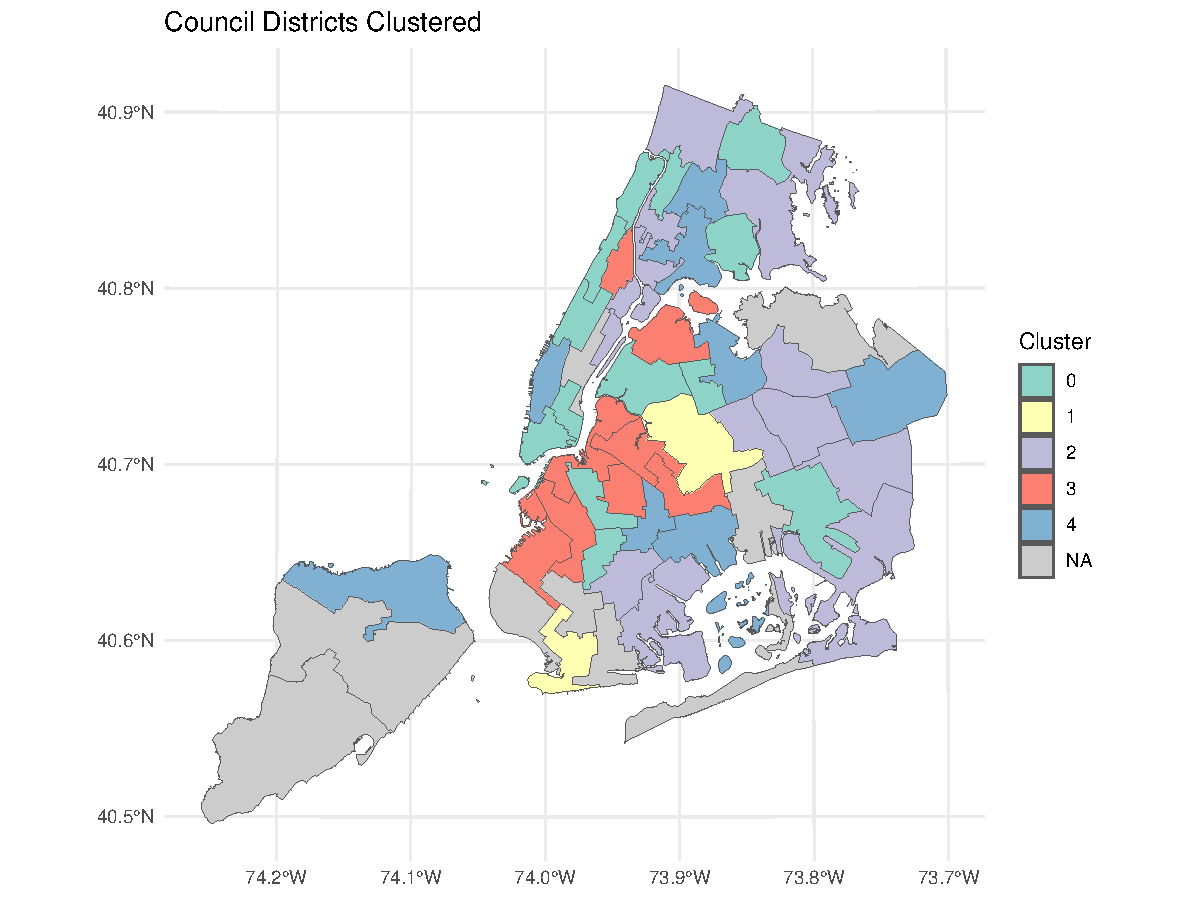
\includegraphics{pdf_test_files/figure-pdf/figure 1-1.pdf}

Cluster 3's homebase is central Brooklyn, with other districts in Harlem
and in northern Queens. A DSA member narrowly lost a race in Brooklyn's
35th district, which would have added to this progressive weight in
central Brooklyn. This location, combined with the demographic
descriptives included above, suggests that the truism of progressive
politics appealing to white, well-educated, economically downwardly
mobile, newcomers may be true, though of course this data is not
granular enough to conclude this. It at least suggests a geographic base
of progressive politics in a diverse and rapidly changing corner of the
city and a broad idea of its demographic characteristics. To dig
further, this section will now turn to the ED level results for the
districts in cluster 3, looking only at the first choice of the RCV.

To further investigate these demographic variables an OLS model was run
on the 919 election districts in which a member of cluster 3 ran, using
vote share for those candidate as its dependent variable. The
independent variables come from two sources, the tract-level ACS 5-Year
file and NYC Open Data, which allows access to datasets from various
city agencies. The variables are the log of the median household income,
the Black and Hispanic share of an ED, the share of non-Hispanic whites
born outside New York State, the share possessing a BA or more, the
share of homeowners, and two variables to register noise complaints. One
noise variables is the average 311 noise complaints per month the other
is the number of noise complaints made during the summer of 2020 when
there was a large spike in many areas of the city. The two variables are
negatively correlated, implying perhaps summer complaint spikes happened
in areas with low average numbers of complaints, so they were both
included. Multicollinearity is a concern with these closely related
demographic variables, but no variable is correlated at a level higher
than .7 or has a VIF higher than 3. The mean and median of all the IVs
are listed below.

\begin{longtable}{rrrrrrrrrrrrrrrrrr}
\toprule
mean\_log & med\_log & mean\_black & med\_black & mean\_hisp & med\_hisp & mean\_wt & med\_wt & mean\_ba & med\_ba & mean\_ho & med\_ho & mean\_snc & med\_snc & mean\_mn & med\_mn & mean\_pr & med\_pr \\ 
\midrule
9.988207 & 10.21516 & 20.64275 & 8.200776 & 27.85176 & 21.63926 & 12.55702 & 10.25325 & 44.99568 & 43.92619 & 24.36346 & 22.49559 & 40.93771 & 30.13977 & 28.26399 & 19.27778 & 9.392132 & 9.397945 \\ 
\bottomrule
\end{longtable}

All variables in the models below have been scaled and standardized to
easily compare effect. While there are some large and significant
effects, the first item of note is that the R squared is quite low.
Additionally, while several of the coefficients point to an electorate
of white, educated, culturally employed, liberal, newcomers, others,
such as education and retail employment did not. Those could be genuine,
the white transplant voting pool could be less educated than imagined or
the EDs these candidates did well in could just be heterogenous (though
the racial variables dispute this).

Dependent variable:

vote\_share

(1)

(2)

(3)

(4)

(5)

log(mhhi21)

-1.714***

-1.415***

-2.078***

-1.731***

-1.609***

(0.455)

(0.452)

(0.460)

(0.470)

(0.467)

nhb21p

-0.371***

-0.354***

-0.275***

-0.329***

-0.331***

(0.030)

(0.029)

(0.032)

(0.035)

(0.034)

h21p

0.183***

0.287***

0.099**

0.082*

(0.036)

(0.040)

(0.044)

(0.044)

white\_transplant\_ratio

0.475***

1.184***

1.183***

(0.084)

(0.145)

(0.143)

cvap21bapp

-0.410***

-0.209**

(0.072)

(0.086)

hh21op

-0.312***

-0.293***

(0.050)

(0.050)

summer\_noise\_complaints

0.057***

0.047**

(0.021)

(0.021)

mean\_noise

-0.082**

-0.050

(0.034)

(0.035)

perc\_retail

2.440***

(0.596)

Constant

66.186***

57.747***

53.871***

73.885***

40.263***

(4.730)

(4.952)

(4.918)

(5.172)

(9.685)

Observations

919

919

919

919

919

R2

0.149

0.173

0.201

0.285

0.298

Adjusted R2

0.147

0.170

0.197

0.279

0.291

Residual Std. Error

20.042 (df = 916)

19.774 (df = 915)

19.448 (df = 914)

18.429 (df = 910)

18.272 (df = 909)

F Statistic

80.248*** (df = 2; 916)

63.609*** (df = 3; 915)

57.324*** (df = 4; 914)

45.389*** (df = 8; 910)

42.905*** (df = 9; 909)

Note:

\emph{p\textless0.1; \textbf{p\textless0.05; }}p\textless0.01

A better explanation seemed to be that one explanation wouldn't fit
every district. To test this a fixed effects model was run using council
districts. R's `fixest' package was used, which includes robust standard
errors and estimates the effects of district indirectly to avoid
multicollinearity. The results are reported in Table 11 below. Now only
income reaches significance at the 95\% confidence level and home
ownership at 90\%. Additionally, the within R2 is very low, only
rounding up to 1\%, while the overall R2 has risen to 56, suggesting
55\% of variance is attributable to variance between districts that
these models don't explain. It appears that these candidates resist a
one size fits all explanation of electoral success.

\begin{table}
\centering
\begin{talltblr}[         %% tabularray outer open
entry=none,label=none,
note{}={+ p &lt; 0.1, * p &lt; 0.05, ** p &lt; 0.01, *** p &lt; 0.001},
]                     %% tabularray outer close
{                     %% tabularray inner open
colspec={Q[]Q[]Q[]Q[]Q[]Q[]},
column{2,3,4,5,6}={}{halign=c,},
column{1}={}{halign=l,},
hline{20}={1,2,3,4,5,6}{solid, black, 0.05em},
}                     %% tabularray inner close
\toprule
& (1) & (2) & (3) & (4) & (5) \\ \midrule %% TinyTableHeader
scale(log_income)              & −2.165  & −2.674* & −2.475* & −2.557** & −2.319* \\
& (2.022) & (0.905) & (0.844) & (0.667)  & (0.810) \\
scale(nhb21p)                  & −3.505+ & −3.426  & −3.610  & −2.884   & −3.090  \\
& (1.628) & (4.880) & (4.708) & (4.331)  & (4.288) \\
scale(h21p)                    &         & −1.248  & −2.184  & −2.271   & −2.410  \\
&         & (5.069) & (5.579) & (5.305)  & (5.340) \\
scale(white_transplant_ratio)  &         & 1.650   & 0.987   & 1.567    & 1.610   \\
&         & (6.140) & (3.759) & (3.799)  & (3.795) \\
scale(cvap21bapp)              &         &         & 0.893   & 3.737    & 3.873   \\
&         &         & (4.374) & (3.265)  & (3.394) \\
scale(hh21op)                  &         &         & −3.642+ & −3.441+  & −3.214+ \\
&         &         & (1.673) & (1.687)  & (1.613) \\
scale(summer_noise_complaints) &         &         &         & 0.218    & −0.545  \\
&         &         &         & (1.160)  & (1.110) \\
scale(perc_retail)             &         &         &         & 3.847    & 4.269   \\
&         &         &         & (2.994)  & (3.078) \\
scale(mean_noise)              &         &         &         &          & 1.650   \\
&         &         &         &          & (1.234) \\
Num.Obs.                       & 919     & 919     & 919     & 919      & 919     \\
R2                             & 0.545   & 0.551   & 0.568   & 0.575    & 0.576   \\
R2 Adj.                        & 0.541   & 0.546   & 0.562   & 0.568    & 0.569   \\
R2 Within                      & 0.032   & 0.045   & 0.081   & 0.095    & 0.098   \\
\bottomrule
\end{talltblr}
\end{table}

\hypertarget{demographic-clustering}{%
\section{Demographic Clustering}\label{demographic-clustering}}

Another approach to understanding the electoral dynamics of this
progressive group is to once again turn to clustering. Since this
progressive group clearly win different groups in different districts,
clustering the council districts and seeing which clusters tend to elect
the progressive bloc can help to tease out electoral patterns. The same
process as above was followed on the same set of demographic predictors
used above, plus some additional categories of ethnicity as well as NYPD
arrest data and primary mode of transportation. All tests used to
determine the proper number of predetermined clusters pointed clearly to
five. Table 12 shows the results for the progressive cluster, cluster 3.
Four of the five demographic clusters are represented by the
progressives. Table 13, directly below, shows the variables that were
the most influential in defining the clusters.

\begin{longtable}{lr}
\toprule
matched\_name & demo\_cluster \\ 
\midrule
Tiffany Caban & 4 \\ 
Jennifer Gutierrez & 4 \\ 
Alexa Aviles & 4 \\ 
Chi A. Osse & 3 \\ 
Kristin Richardson Jordan & 2 \\ 
Sandy Nurse & 2 \\ 
Lincoln Restler & 1 \\ 
Shahana K. Hanif & 1 \\ 
\bottomrule
\end{longtable}

\begin{longtable}{lllll}
\caption*{
{\large Top Variables and Scores for Each Cluster} \\ 
{\small Ranked by Importance}
} \\ 
\toprule
Cluster 0 & Cluster 1 & Cluster 2 & Cluster 3 & Cluster 4 \\ 
\midrule
kor21p (3.49) & white\_transplant\_ratio (1.91) & domin21p (1.48) & winda21p (1.75) & colomb21p (0.87) \\ 
nha21p (2.48) & perc\_finance (1.85) & mean\_noise (1.28) & black\_fb\_ratio (1.69) & rv21italp (0.71) \\ 
chin21p (2.33) & wfh\_ratio (1.75) & prican21p (1.08) & nhb21p (1.62) & mex21p (0.68) \\ 
train\_ratio (1.55) & cvap21bapp (1.71) & hh21rc (1.08) & black\_nys\_ratio (1.43) & venez21p (0.56) \\ 
drive\_ratio (1.54) & walk\_ratio (1.61) & summer\_noise\_complaints (1.05) & perc\_healthcare (0.95) & ldensity (0.54) \\ 
p21own (1.46) & same\_sex\_ratio (1.57) & femHHH\_ratio (0.98) & femHHH\_ratio (0.79) & mean\_arrests (-0.52) \\ 
bike\_ratio (-0.84) & bike\_ratio (1.51) & nha21p (-0.72) & mex21p (-0.70) & winda21p (-0.55) \\ 
mex21p (-0.85) & nhw21p (1.47) & nhw21p (-0.78) & nhw21p (-0.75) & black\_fb\_ratio (-0.65) \\ 
black\_nys\_ratio (-0.90) & perc\_healthcare (-1.45) & p21own (-1.04) & walk\_ratio (-0.76) & nhb21p (-0.71) \\ 
mean\_arrests (-1.15) & perc\_retail (-1.73) & mhhi21 (-1.21) & rv21italp (-1.00) & black\_nys\_ratio (-0.71) \\ 
\bottomrule
\end{longtable}

The demographic heterogeneity of the districts sheds light on why the
models above had low explanatory power. Income and broad racial
categories are the only variables that all districts have in common. In
the next several chapters each district and candidate will be explored
in more detail, but for the time being Table 14 below shows models fit
on each cluster. Model one corresponds to cluster one, etc. The R
squared values have risen significantly, and different variables
evidently effect the outcome of progressive candidates differently. In
the whiter and wealthier cluster 1 it is indeed the poorer districts
that votes for the progressive. In the poorer and more Black and
Hispanic cluster 4 (where both DSA candidates won) income has less of an
effect but white transplants clearly do.\\

Dependent variable:

Cluster 1

(1)

(2)

(3)

(4)

log\_income

-2.828***

1.395

1.789

0.293

(0.686)

(1.127)

(4.079)

(1.771)

nhb21p

-5.865*

8.386***

-4.349

1.753

(3.258)

(2.241)

(4.528)

(2.401)

h21p

-13.840***

10.738***

-9.375**

8.364***

(2.600)

(1.648)

(4.211)

(1.096)

white\_transplant\_ratio

-3.292

36.984***

7.339*

14.357***

(2.282)

(4.186)

(4.418)

(1.515)

cvap21bapp

-7.266**

-8.149***

-1.007

3.383

(2.881)

(3.068)

(4.513)

(2.186)

hh21op

-6.831***

2.312*

0.056

-3.090***

(1.225)

(1.324)

(1.759)

(0.899)

summer\_noise\_complaints

-1.700

0.694

0.445

-2.001

(1.751)

(1.150)

(3.007)

(1.240)

mean\_noise

-1.505

-3.488***

7.918**

7.956***

(2.705)

(1.134)

(3.913)

(1.548)

perc\_retail

-4.164*

6.217***

-0.708

2.110

(2.133)

(1.960)

(2.351)

(1.920)

Constant

35.858***

38.146***

36.680***

51.965***

(2.537)

(2.421)

(4.053)

(1.804)

Observations

257

237

115

310

R2

0.466

0.497

0.560

0.677

Adjusted R2

0.446

0.477

0.523

0.667

Residual Std. Error

14.628 (df = 247)

13.903 (df = 227)

9.557 (df = 105)

12.733 (df = 300)

F Statistic

23.920*** (df = 9; 247)

24.955*** (df = 9; 227)

14.863*** (df = 9; 105)

69.788*** (df = 9; 300)

Note:

\emph{p\textless0.1; \textbf{p\textless0.05; }}p\textless0.01



\end{document}
